\documentclass{standalone}

\usepackage{pgfplots}

\usetikzlibrary{fit,positioning}
\usetikzlibrary{calc,positioning,shapes.geometric}
\usetikzlibrary{arrows.meta}

\tikzset{>={Latex[width=2mm,length=1mm]}}

\begin{document}

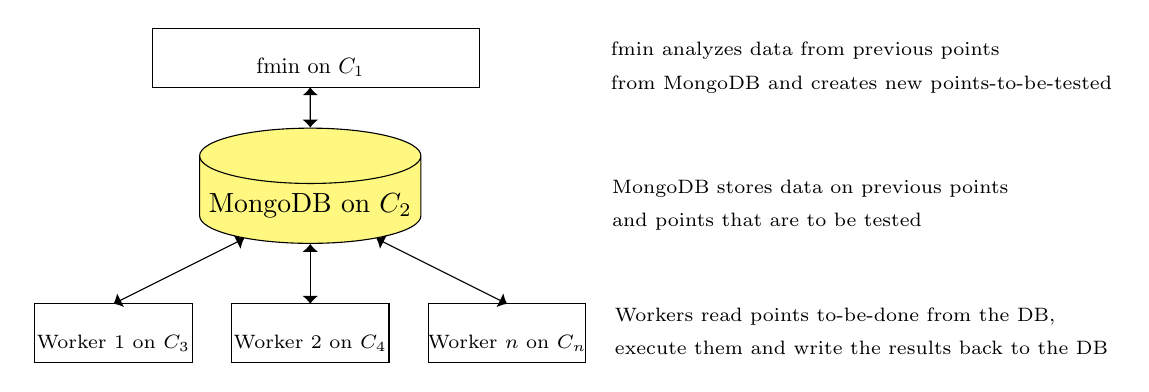
\begin{tikzpicture}[
    scale=0.5,
    database/.style={
        cylinder,
        cylinder uses custom fill,
        cylinder body fill=yellow!50,
        cylinder end fill=yellow!50,
        shape border rotate=90,
        aspect=0.25,
        draw
    }
]

\draw (3,0) -- (3,1.5) -- (11.3,1.5) -- (11.3,0) -- cycle;
\node[scale=0.8] (fmin) at (7,0.5) {fmin on $C_1$};
\node[align=left] (fmincomment) at (21, 0.5) {\scriptsize fmin analyzes data from previous points\\\scriptsize from MongoDB and creates new points-to-be-tested};

\node[database] (db) at (7,-3) {MongoDB on $C_2$};
\node[align=left] (dbcomment) at (19.7, -3) {\scriptsize MongoDB stores data on previous points\\\scriptsize and points that are to be tested};

\coordinate (fmincenter) at (7, 0);

\draw[<->] (fmincenter) -- (db);

\draw (0,-7) -- (0,-5.5) -- (4,-5.5) -- (4,-7) -- cycle ;
\node (w1) at (2,-6.5) {\scriptsize Worker 1 on $C_3$};
\coordinate (w1center) at (2,-5.5);

\draw (5,-7) -- (5,-5.5) -- (9,-5.5) -- (9,-7) -- cycle ;
\node (w2) at (7,-6.5) {\scriptsize Worker 2 on $C_4$};
\coordinate (w2center) at (7,-5.5);

\draw (10,-7) -- (10,-5.5) -- (14,-5.5) -- (14,-7) -- cycle;
\node (wn) at (12,-6.5) {\scriptsize Worker $n$ on $C_{n}$};
\coordinate (wncenter) at (12,-5.5);

\node[align=left] (workerscomment) at (21, -6.2) {\scriptsize Workers read points to-be-done from the DB,\\\scriptsize execute them and write the results back to the DB};

\draw[<->] (db) -- (w1center);
\draw[<->] (db) -- (w2center);
\draw[<->] (db) -- (wncenter);

\end{tikzpicture}

\end{document}
